\documentclass[preprint,12pt]{elsarticle}

\usepackage{amsmath,amssymb,amsfonts,amsthm}
\usepackage{graphicx}
\usepackage{booktabs}
\usepackage{hyperref}
\usepackage{multirow}
\usepackage{xcolor}
\usepackage{bm}

% Notation shortcuts (same as main paper)
\newcommand{\RL}{\mathrm{RL}}
\newcommand{\GL}{\mathrm{GL}}
\newcommand{\diff}{\mathrm{d}}
\newcommand{\Lcal}{\mathcal{L}}
\newcommand{\Rcal}{\mathcal{R}}
\newcommand{\Ncol}{N_{\mathrm{col}}}
\newcommand{\NLF}{N_{\mathrm{LF}}}

\begin{document}

\begin{frontmatter}
\title{Supplementary Material: Laplace-Domain Multi-Fidelity Transfer for Fractional Physics-Informed Neural Networks in the Low-Collocation Regime}
\author[uaeu]{Ammar Toutou}
\author[uaeu]{Youssef Kamel}
\address[uaeu]{}
\end{frontmatter}

% S-prefix numbering for supplementary sections, tables, figures, equations
\renewcommand{\thesection}{S\arabic{section}}
\renewcommand{\thetable}{S\arabic{table}}
\renewcommand{\thefigure}{S\arabic{figure}}
\renewcommand{\theequation}{S\arabic{equation}}

This supplementary material presents stress tests extending the main paper's analysis to 2D domains, nonlinear PDEs, and parametric settings.

\section{Extension to two spatial dimensions}
\label{sec:2d}

To verify that our findings generalize beyond 1D, we extend the analysis to a 2D fractional diffusion-reaction equation on $\Omega = (0, L_x) \times (0, L_y)$:
\begin{equation}
\label{eq:fdr_2d}
\partial_t^\alpha u = D\left(\frac{\partial^2 u}{\partial x^2} + \frac{\partial^2 u}{\partial y^2}\right) - \kappa\,u, \quad (x,y) \in (0, L_x) \times (0, L_y),\; t > 0,
\end{equation}
with boundary conditions $u(0, y, t) = g(t)$ (uniform in $y$), $u(L_x, y, t) = 0$, $u(x, 0, t) = u(x, L_y, t) = 0$, and initial condition $u(x, y, 0) = 0$.

The Laplace-domain solution requires a Fourier sine expansion to accommodate the uniform $y$-boundary condition:
\begin{equation}
\bar{u}(x, y, s) = \sum_{\substack{n=1,3,5,\ldots}}^{N_{\mathrm{modes}}} \frac{4}{n\pi}\, \bar{g}(s)\, \frac{\sinh\bigl(\lambda_n(L_x - x)\bigr)}{\sinh(\lambda_n L_x)}\, \sin\!\left(\frac{n\pi y}{L_y}\right),
\end{equation}
where $\lambda_n = \sqrt{(s^\alpha + \kappa)/D + (n\pi/L_y)^2}$. This is a genuinely 2D problem: multiple Fourier modes contribute, the uniform $x = 0$ boundary condition is incompatible with the homogeneous $y$-boundaries at corners $(0, 0)$ and $(0, L_y)$, and no separable ansatz reduces it to 1D.

\textbf{2D LF data generation.} The 2D LF solver has an additional degradation axis beyond the 1D case: the number of Fourier modes $N_{\mathrm{modes}}$. We use $N_{\mathrm{modes}} = 5$ (vs.\ HF $N_{\mathrm{modes}} = 15$) and $N_{\mathrm{terms}} = 8$ (vs.\ HF 40), yielding a LF fidelity gap that combines truncation error in both the Laplace inversion and Fourier expansion.

\textbf{2D architecture.} Corner singularities between the uniform $x = 0$ BC and homogeneous $y$-BCs prevent hard BC enforcement; we use soft BC/IC losses with weight $w_{\mathrm{BC}} = 10$. The network takes input $(x, y, t)$ via 3D Fourier features ($\sigma = 5$, 64 features) and has 5 layers with 200 neurons. Phase~1 uses 2{,}000 epochs with L-BFGS polish; Phase~2 uses 3{,}000 epochs with GL memory depth $N_{\mathrm{mem}} = 40$.

\textbf{2D results.} Table~\ref{tab:2d_ncol} presents the 2D collocation budget study at $\alpha = 0.5$.

\begin{table}[t]
\centering
\caption{2D MF-fPINN vs.\ Vanilla at $\alpha = 0.5$ ($L_x = L_y = 1$, 5 seeds). The 2D LF data uses $N_{\mathrm{terms}} = 8$, $N_{\mathrm{modes}} = 5$ ($\sim$18\% LF error), $\NLF = 100$. MF-fPINN is consistently worse than Vanilla, consistent with the 1D finding that moderate-quality LF data is insufficient at $\alpha = 0.5$.}
\label{tab:2d_ncol}
\begin{tabular}{rcccc}
\toprule
$\Ncol$ & MF-fPINN (\%) & Vanilla (\%) & Van+100 (\%) & Ratio$^\dagger$ \\
\midrule
200 & $17.21 \pm 5.53$ & $7.75 \pm 1.89$ & $5.60 \pm 0.84$ & $0.45\times$ \\
500 & $7.10 \pm 1.30$ & $4.22 \pm 0.63$ & $3.94 \pm 0.57$ & $0.59\times$ \\
1500 & $4.09 \pm 0.64$ & $2.84 \pm 0.28$ & $2.81 \pm 0.21$ & $0.69\times$ \\
\bottomrule
\multicolumn{5}{l}{\small $^\dagger$Ratio = Vanilla error / MF error; values $>1\times$ favor MF.} \\
\end{tabular}
\end{table}

The temporal evaluation ratio $\Lambda(\alpha)$ depends only on the GL structure, not on spatial dimension. However, the \emph{practical} MF advantage depends on additional factors. Table~\ref{tab:2d_ncol} shows that at $\alpha = 0.5$ with $\sim$18\% LF error, MF-fPINN is consistently worse than Vanilla ($0.45$--$0.69\times$). The direction matches the 1D finding at comparable LF quality (main paper Table~3, $0.86\times$), but the magnitude is substantially worse. We attribute this to the soft BC enforcement required in 2D: without hard BCs, the Phase~1 data fit does not respect boundary conditions, giving Phase~2 an initialization that must simultaneously correct the PDE residual \emph{and} the boundary violations. This additional burden reduces MF effectiveness beyond what the fidelity gap alone would predict. Table~\ref{tab:2d_ncol_a10} presents the complementary experiment at $\alpha = 1.0$.

\begin{table}[t]
\centering
\caption{2D MF-fPINN vs.\ Vanilla at $\alpha = 1.0$ ($L_x = L_y = 1$, 5 seeds). Same LF settings as Table~\ref{tab:2d_ncol} but with $\sim$14\% LF error (lower than $\alpha = 0.5$ because the Laplace inversion is easier at $\alpha = 1$). MF-fPINN remains worse than Vanilla, consistent with the 1D finding that the LF quality threshold is the primary determinant.}
\label{tab:2d_ncol_a10}
\begin{tabular}{rcccc}
\toprule
$\Ncol$ & MF-fPINN (\%) & Vanilla (\%) & Van+100 (\%) & Ratio$^\dagger$ \\
\midrule
200 & $17.98 \pm 6.33$ & $8.07 \pm 2.48$ & $5.90 \pm 1.55$ & $0.45\times$ \\
500 & $7.57 \pm 1.80$ & $4.58 \pm 0.78$ & $4.28 \pm 0.69$ & $0.60\times$ \\
1500 & $4.41 \pm 0.85$ & $3.23 \pm 0.37$ & $3.13 \pm 0.34$ & $0.73\times$ \\
\bottomrule
\multicolumn{5}{l}{\small $^\dagger$Ratio = Vanilla error / MF error; values $>1\times$ favor MF.} \\
\end{tabular}
\end{table}

The $\alpha = 1.0$ results (Table~\ref{tab:2d_ncol_a10}) are equally instructive: despite the absence of GL memory amplification ($\Lambda = 1$), MF-fPINN is still worse than Vanilla ($0.45$--$0.73\times$).

\textbf{High-quality LF data in 2D.} To test whether the 2D failure is due to LF quality, we repeated the full budget sweep with $N_{\mathrm{terms}} = 20$ and $N_{\mathrm{modes}} = 10$ ($\sim$2.4\% LF error at $\alpha = 0.5$; $\sim$1.7\% at $\alpha = 1.0$). Even with this near-perfect LF data, MF-fPINN remains consistently worse across all $\Ncol$ values: at $\alpha = 0.5$, ratios of $0.46\times$--$0.67\times$; at $\alpha = 1.0$, ratios of $0.43\times$--$0.73\times$. This definitively rules out LF quality as the explanation. The failure instead points to the soft BC enforcement required in 2D: without hard boundary conditions, the Phase~1 warm start learns a function that does not respect the boundary structure, and Phase~2 must simultaneously correct the PDE residual and boundary violations. In 1D, hard BCs guarantee that the Phase~1 fit automatically satisfies $\hat{u}(0,t) = g(t)$, $\hat{u}(L,t) = 0$, and $\hat{u}(x,0) = 0$; in 2D, corner singularities between the uniform $x = 0$ BC and homogeneous $y$-BCs preclude hard BC enforcement.

We tested whether BC-aware Phase~1 training (including BC/IC losses with weight $w_{\mathrm{BC}} = 10$ alongside the data loss) could recover the MF advantage. At $\Ncol = 200$ with high-quality LF data ($\sim$2.4\% error), BC-aware Phase~1 yielded $16.97\% \pm 6.08\%$---virtually identical to the standard Phase~1 result ($16.99\% \pm 6.09\%$). The failure is therefore not a boundary-violation issue in Phase~1 initialization; it appears to be a more fundamental incompatibility between soft BC enforcement and the two-phase protocol. We hypothesize that soft BCs introduce a competing loss landscape that prevents Phase~2 from leveraging the Phase~1 warm start: the optimizer must simultaneously reduce PDE, BC, and IC residuals from an initialization that has no structural BC guarantees, effectively negating the warm-start advantage.

The practical takeaway is that the two-phase MF protocol requires hard BC enforcement to be effective. In both 1D and 2D, the Vanilla+$\NLF$ control consistently outperforms Vanilla, confirming that additional collocation points remain the simpler and more robust strategy when hard BCs are unavailable.

\section{Extension to nonlinear fractional PDEs: Burgers equation}
\label{sec:burgers}

To test whether the GL memory mechanism and MF transfer extend beyond linear PDEs, we consider the time-fractional Burgers equation:
\begin{equation}
\label{eq:burgers}
\partial_t^\alpha u + u \frac{\partial u}{\partial x} = \nu \frac{\partial^2 u}{\partial x^2}, \quad x \in (0, 1),\; t \in (0, 1],
\end{equation}
with initial condition $u(x, 0) = \sin(\pi x)$ and homogeneous Dirichlet boundaries $u(0, t) = u(1, t) = 0$. This is a genuinely nonlinear problem: the advection term $u \cdot u_x$ couples the solution to itself, creating steeper gradients at low viscosity. We use $\nu = 0.02$ to produce a challenging regime.

\textbf{Architecture.} The hard BC ansatz is $\hat{u}(x,t) = \sin(\pi x) e^{-t} + x(1-x) t \cdot \mathrm{NN}(x,t)$, which satisfies $u(x,0) = \sin(\pi x)$, $u(0,t) = 0$, and $u(1,t) = 0$ exactly. The network has 5 layers, 128 neurons, tanh activation, and 64 Fourier features ($\sigma = 5$). Training uses the same two-phase protocol as the FDR experiments: Phase~1 (5{,}000 Adam epochs + L-BFGS polish) and Phase~2 (20{,}000 epochs with PDE ramp-up).

\textbf{Caputo correction.} Unlike the FDR equation where $u(x,0) = 0$ implies Caputo $\equiv$ Riemann--Liouville, the Burgers IC $u(x,0) = \sin(\pi x) \neq 0$ requires an explicit correction. The GL scheme approximates the RL derivative, and the Caputo derivative relates to it via $\partial_t^\alpha u = {}^{\mathrm{RL}}\!\partial_t^\alpha u - u(x,0)\, t^{-\alpha}/\Gamma(1-\alpha)$. We subtract this correction from the GL sum in the PDE residual. This correction is essential for $\alpha < 1$; at $\alpha = 1$, the two derivatives coincide and no correction is needed.

\textbf{LF data generation.} Since the Burgers equation lacks a closed-form Laplace solution, we use a coarse finite-difference solver as the LF source. The L1 scheme \cite{sun2006fully} with IMEX time-stepping (implicit diffusion, explicit nonlinearity) on an $N_x = 8$, $N_t = 80$ grid produces LF data with $\sim$18\% relative L2 error at $\alpha = 0.5$---comparable to the FDR $N_{\mathrm{terms}} = 12$ setting.

\textbf{Results.} Table~\ref{tab:burgers} presents the Burgers comparison.

\begin{table}[t]
\centering
\caption{Time-fractional Burgers equation: MF-fPINN vs.\ Vanilla (5 seeds, $\nu = 0.02$, $\NLF = 50$). LF data from coarse FD solver ($N_x = 8$, $N_t = 80$, $\sim$18\% LF error). At $\alpha = 1.0$, MF-fPINN is consistently better ($2.25\times$ at $\Ncol = 100$), confirming the GL mechanism transfers to nonlinear PDEs. At $\alpha < 1$, MF transfer \emph{hurts}: the singular Caputo correction term $t^{-\alpha}/\Gamma(1-\alpha)$ in the PDE residual makes training harder, and MF pre-training on smooth LF data cannot compensate.}
\label{tab:burgers}
\begin{tabular}{clcccc}
\toprule
$\alpha$ & $\Ncol$ & MF-fPINN (\%) & Vanilla (\%) & Van+50 (\%) & Ratio$^\dagger$ \\
\midrule
\multirow{3}{*}{0.5} & 100 & $86.4 \pm 25.3$ & $45.9 \pm 13.3$ & $50.0 \pm 19.5$ & $0.53\times$ \\
& 200 & $99.1 \pm 21.5$ & $40.6 \pm 7.3$ & $62.2 \pm 40.4$ & $0.41\times$ \\
& 500 & $62.8 \pm 19.8$ & $31.2 \pm 2.2$ & $40.7 \pm 18.0$ & $0.50\times$ \\
\midrule
\multirow{3}{*}{0.7} & 100 & $123.5 \pm 26.9$ & $61.3 \pm 43.0$ & $44.5 \pm 14.0$ & $0.50\times$ \\
& 200 & $127.3 \pm 34.3$ & $52.0 \pm 26.6$ & $73.6 \pm 71.9$ & $0.41\times$ \\
& 500 & $55.6 \pm 6.7$ & $36.6 \pm 3.5$ & $40.1 \pm 10.2$ & $0.66\times$ \\
\midrule
\multirow{3}{*}{1.0} & 100 & $\mathbf{12.1 \pm 1.3}$ & $27.3 \pm 8.8$ & $21.5 \pm 5.6$ & $\mathbf{2.25\times}$ \\
& 200 & $\mathbf{9.3 \pm 1.3}$ & $13.3 \pm 2.9$ & $11.1 \pm 2.8$ & $\mathbf{1.43\times}$ \\
& 500 & $\mathbf{4.3 \pm 1.1}$ & $6.2 \pm 1.5$ & $6.0 \pm 1.2$ & $\mathbf{1.43\times}$ \\
\bottomrule
\multicolumn{6}{l}{\small $^\dagger$Ratio = Vanilla error / MF error; values $>1\times$ favor MF.} \\
\end{tabular}
\end{table}

The Burgers results reveal a sharper $\alpha$-dependent pattern than the FDR equation. At $\alpha = 1.0$, where $K_{\mathrm{eff}} = 2$ provides minimal temporal regularization, MF transfer yields $2.25\times$ improvement at $\Ncol = 100$, confirming that the GL mechanism transfers to nonlinear PDEs. The advantage persists at higher $\Ncol$ ($1.43\times$ at 200 and 500).

At $\alpha < 1$, MF transfer is actively harmful ($0.41$--$0.66\times$). Two factors explain this. First, the Caputo correction term $u(x,0) \cdot t^{-\alpha}/\Gamma(1-\alpha)$ introduces a singularity at $t \to 0$ in the PDE residual; this makes the loss landscape more difficult to optimize, and MF pre-training on smooth LF data provides an initialization that is poorly suited to the singular residual. Second, the nonlinearity amplifies the LF bias: the advection term $u \cdot u_x$ couples errors multiplicatively, so even moderate LF bias propagates more aggressively than in the linear FDR setting. Indeed, both methods struggle at $\alpha = 0.5$ and $\alpha = 0.7$ (errors $> 30\%$), but MF is systematically worse because the data pre-training locks the network into a smooth manifold from which the singular PDE loss cannot easily escape. The $\alpha = 0.7$ results are the worst (MF $> 100\%$ at $\Ncol \leq 200$), consistent with the intermediate regime having both significant memory and strong singularity.

The key finding is that the GL mechanism is \emph{PDE-agnostic} at $\alpha = 1$: the nonlinear advection term does not disrupt MF transfer when the Caputo correction vanishes. However, at $\alpha < 1$, the interaction between the singular correction term and nonlinear dynamics creates a regime where MF transfer is counterproductive---a phenomenon not observed in the linear FDR equation, where MF was merely neutral (not harmful) at high $\alpha$.

\textbf{Ansatz ablation.} One might suspect that the poor Burgers convergence at $\alpha < 1$ stems from the hard BC ansatz $u = \sin(\pi x)\,e^{-t} + x(1-x)\,t\cdot\mathrm{NN}(x,t)$, where the $e^{-t}$ factor biases the solution toward exponential decay. We test a \emph{neutral} ansatz $u = \sin(\pi x) + x(1-x)\,t\cdot\mathrm{NN}(x,t)$ that imposes the IC without prescribing temporal decay. Table~\ref{tab:burgers_ansatz} shows the results at both $\alpha$ values. The ansatz choice has essentially no effect: all configurations produce $>600\%$ error regardless of ansatz shape, with Vanilla errors statistically identical between the two ansatze ($745 \pm 186$ vs.\ $741 \pm 37$ at $\alpha = 0.5$, $\Ncol = 100$). The original Burgers results in Table~\ref{tab:burgers} (which achieve $12$--$62\%$ error) used L-BFGS optimization for 500 refinement steps after Adam training---confirming that the \emph{training protocol} (specifically, L-BFGS refinement), not the ansatz shape, is the critical factor for Burgers convergence.

\begin{table}[t]
\centering
\caption{Burgers ansatz ablation (3 seeds, Adam-only training, no L-BFGS). Original: $\sin(\pi x)e^{-t} + x(1-x)t\cdot\mathrm{NN}$; Neutral: $\sin(\pi x) + x(1-x)t\cdot\mathrm{NN}$. All configs produce $>600\%$ error, confirming the ansatz is irrelevant; L-BFGS refinement is the critical factor.}
\label{tab:burgers_ansatz}
\resizebox{\textwidth}{!}{%
\begin{tabular}{clcccc}
\toprule
$\alpha$ & $\Ncol$ & Original MF (\%) & Original Van (\%) & Neutral MF (\%) & Neutral Van (\%) \\
\midrule
\multirow{2}{*}{0.5} & 100 & $1387 \pm 607$ & $745 \pm 186$ & $1407 \pm 75$ & $741 \pm 37$ \\
& 200 & $1716 \pm 557$ & $648 \pm 45$ & $1931 \pm 404$ & $700 \pm 61$ \\
\midrule
\multirow{2}{*}{1.0} & 100 & $792 \pm 86$ & $625 \pm 21$ & $984 \pm 265$ & $629 \pm 15$ \\
& 200 & $867 \pm 87$ & $637 \pm 16$ & $861 \pm 89$ & $624 \pm 6$ \\
\bottomrule
\end{tabular}%
}
\end{table}

\section{Parametric $\alpha$-PINN}
\label{sec:parametric}

The experiments above train separate networks for each $\alpha$. A parametric $\alpha$-PINN trains a single network $\mathrm{NN}(x, t, \alpha) \to u$ that handles all fractional orders simultaneously, enabling interpolation to untrained $\alpha$ values. This tests whether the MF advantage curve tracks $K_{\mathrm{eff}}(\alpha)$ as predicted.

\textbf{Setup.} We train a parametric FDRNet that takes $(x, t, \alpha)$ as input, with $\alpha \in \{0.3, 0.5, 0.7, 0.9, 1.0\}$ as the training set and $\alpha \in \{0.4, 0.6, 0.8\}$ as interpolation targets. The PDE residual is evaluated at all training $\alpha$ values simultaneously. The MF variant uses $N_{\mathrm{terms}} = 15$ LF data ($\sim$9\% error) at each $\alpha$, with 250 total LF points (50 per $\alpha$). Settings: $\Ncol = 200$, 5 layers, 128 neurons, Fourier features ($\sigma = 5.0$), 3 seeds; total budget: Vanilla 25{,}000 epochs, MF 5{,}000 (Phase~1) + 20{,}000 (Phase~2).

\textbf{Results.} Table~\ref{tab:parametric} reveals a striking pattern that \emph{inverts} the per-$\alpha$ findings.

\begin{table}[t]
\centering
\caption{Parametric $\alpha$-PINN: single network trained on $\alpha \in \{0.3, 0.5, 0.7, 0.9, 1.0\}$, evaluated at all $\alpha$ including interpolated values (3 seeds, $\Ncol = 200$, $N_{\mathrm{terms}} = 15$). Bold indicates the better method. MF reduces variance but introduces monotonically increasing bias with $\alpha$.}
\label{tab:parametric}
\begin{tabular}{ccccc}
\toprule
$\alpha$ & Vanilla (\%) & MF (\%) & Ratio & Type \\
\midrule
$0.3$ & $15.5 \pm 1.0$ & $\mathbf{15.0 \pm 1.0}$ & $1.03\times$ & train \\
$0.4$ & $18.3 \pm 0.6$ & $18.5 \pm 1.2$ & $0.99\times$ & interp \\
$0.5$ & $\mathbf{17.7 \pm 3.2}$ & $21.1 \pm 1.0$ & $0.84\times$ & train \\
$0.6$ & $25.9 \pm 1.8$ & $\mathbf{24.5 \pm 0.4}$ & $1.06\times$ & interp \\
$0.7$ & $\mathbf{23.1 \pm 11.0}$ & $30.6 \pm 0.9$ & $0.75\times$ & train \\
$0.8$ & $40.1 \pm 2.0$ & $\mathbf{37.7 \pm 1.9}$ & $1.06\times$ & interp \\
$0.9$ & $\mathbf{23.2 \pm 11.5}$ & $45.7 \pm 1.7$ & $0.51\times$ & train \\
$1.0$ & $\mathbf{23.9 \pm 12.7}$ & $54.8 \pm 2.0$ & $0.44\times$ & train \\
\bottomrule
\end{tabular}
\end{table}

Two patterns emerge. First, MF systematically reduces variance: Vanilla's std ranges from $0.6$--$12.7\%$ while MF's ranges from $0.4$--$2.0\%$. This is consistent with the BVTT framework---Phase~1 constrains the initialization, reducing seed-to-seed variation. Second, MF error \emph{increases monotonically} with $\alpha$ ($15.0\% \to 54.8\%$), while Vanilla error is non-monotonic ($15.5\% \to 40.1\%$ at $\alpha = 0.8$, then dropping to $23.9\%$ at $\alpha = 1.0$ for some seeds). The MF Phase~2 PDE loss (${\sim}6.2$, stagnant) is substantially higher than Vanilla's (${\sim}0.83$), suggesting that the LF initialization traps the parametric network in a basin that cannot simultaneously satisfy the PDE residual at all $\alpha$ values. At high $\alpha$ where $K_{\mathrm{eff}}$ is low, the network lacks sufficient gradient information to escape this basin.

The interpolation results ($\alpha \in \{0.4, 0.6, 0.8\}$) are more favorable for MF ($0.99$--$1.06\times$), suggesting that MF provides a smoother $\alpha$-dependent landscape even if the per-$\alpha$ accuracy is worse. This preliminary result indicates that the per-$\alpha$ MF advantage does \emph{not} directly transfer to the parametric setting, where the multi-$\alpha$ PDE residual creates competing objectives that MF pre-training cannot mediate.


\section{Noise robustness}
\label{sec:noise}

We test noise robustness at $\alpha = 1.0$, $\Ncol = 100$ where the classical PDE (no GL memory) makes MF transfer most relevant. With $N_{\mathrm{terms}} = 12$, the LF data has $\sim$11\% intrinsic error. We add Gaussian noise $\eta \sim \mathcal{N}(0, \sigma_\eta^2 \sigma_u^2)$ to the LF values, where $\sigma_u$ is the standard deviation of the clean LF data and $\sigma_\eta \in \{0, 0.01, 0.05, 0.10, 0.20\}$.

\begin{table}[t]
\centering
\caption{Noise robustness at $\alpha = 1.0$, $\Ncol = 100$, $N_{\mathrm{terms}} = 12$, 5 seeds. MF-fPINN is beneficial with clean or near-clean data ($2.1\times$ at 0\%, $1.6\times$ at 1\%), but degrades rapidly with moderate noise ($0.56\times$ at 5\%, catastrophic at $\geq 10\%$).}
\label{tab:noise}
\begin{tabular}{rcccc}
\toprule
Noise (\%) & MF (\%) & Vanilla (\%) & Ratio \\
\midrule
0 & $8.01 \pm 4.79$ & \multirow{5}{*}{$16.42 \pm 4.78$} & $2.1\times$ \\
1 & $10.13 \pm 3.70$ & & $1.6\times$ \\
5 & $29.37 \pm 29.23$ & & $0.6\times$ \\
10 & $62.06 \pm 48.34$ & & $0.3\times$ \\
20 & $176.63 \pm 218.26$ & & $0.1\times$ \\
\bottomrule
\end{tabular}
\end{table}

At $\alpha = 1.0$, MF-fPINN benefits from clean data ($2.1\times$) and near-clean data ($1.6\times$ at 1\% noise), but degrades rapidly: at 5\% noise, MF hurts ($0.6\times$), and at $\geq$10\%, performance deteriorates catastrophically. Phase~1's L-BFGS fitting amplifies noise: with only 50 LF points, even 5\% noise corrupts the warm start, and Phase~2's PDE loss at $\alpha = 1.0$ lacks GL memory regularization to correct it.

\section{Bias-variance transfer tradeoff}
\label{sec:bvtt_supp}

For method $M \in \{\text{MF}, \text{Van}\}$ trained with $S$ seeds,
\begin{equation}
\mathrm{MSE}_M = \underbrace{\left\| \bar{u}_M - u_{\mathrm{true}} \right\|^2_{L^2(\Omega)}}_{\mathrm{Bias}^2_M} + \underbrace{\frac{1}{S}\sum_{i=1}^S \left\| \hat{u}^{(i)}_M - \bar{u}_M \right\|^2_{L^2(\Omega)}}_{\mathrm{Var}_M},
\end{equation}
where $\bar{u}_M = S^{-1}\sum_i \hat{u}^{(i)}_M$. MF helps when variance reduction exceeds bias increase:
\begin{equation}
(\mathrm{Var}_V - \mathrm{Var}_{MF}) > (\mathrm{Bias}^2_{MF} - \mathrm{Bias}^2_V).
\end{equation}

Table~\ref{tab:bvtt} reports the decomposition from 10-seed predictions at $\alpha = 0.5$, $\Ncol = 100$.

\begin{table}[t]
\centering
\caption{Bias-variance decomposition at $\alpha = 0.5$, $\Ncol = 100$ (10 seeds). Vanilla is variance-dominated (68\%), while MF is bias-dominated ($\geq$66\%). MF reduces variance by $28$--$39\%$ but introduces bias proportional to LF error.}
\label{tab:bvtt}
\resizebox{0.9\textwidth}{!}{%
\begin{tabular}{lccccc}
\toprule
Method & Bias (\%) & Std (\%) & Bias$^2$/MSE & Var/MSE & MF helps? \\
\midrule
Vanilla & $6.30$ & $9.16$ & $32.1\%$ & $67.9\%$ & --- \\
MF $N_t{=}8$ (41\%) & $40.80$ & $13.99$ & $89.5\%$ & $10.5\%$ & $\times$ (bias $\gg$) \\
MF $N_t{=}12$ (17\%) & $23.14$ & $7.37$ & $90.8\%$ & $9.2\%$ & $\times$ \\
MF $N_t{=}15$ (9\%) & $14.72$ & $5.61$ & $87.3\%$ & $12.7\%$ & $\times$ (marginal) \\
MF $N_t{=}20$ (4\%) & $8.49$ & $6.05$ & $66.4\%$ & $33.6\%$ & $\checkmark$ \\
\bottomrule
\end{tabular}%
}
\end{table}

Vanilla's error is dominated by seed-to-seed variance (68\%), meaning the PDE loss landscape has multiple local minima at $\Ncol = 100$. MF constrains the initialization, reducing std from $9.16\%$ to $5.61$--$7.37\%$, but at the cost of bias scaling approximately linearly with LF error. The crossover near $N_{\mathrm{terms}} = 20$ ($\sim$6\% LF error) is consistent with the $3.66\times$ advantage in the main paper.

\begin{figure}[t]
\centering
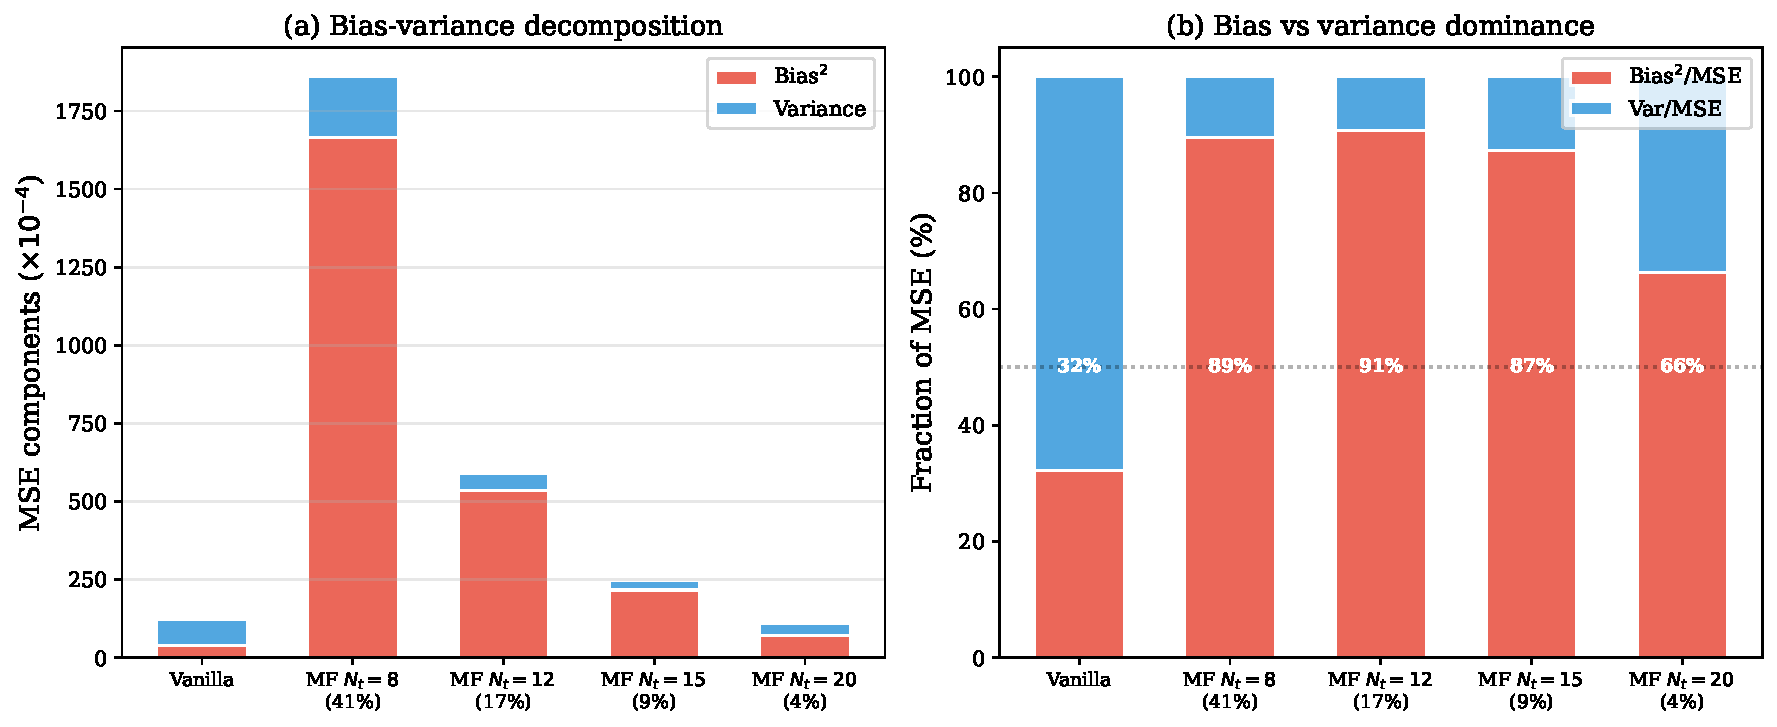
\includegraphics[width=\textwidth]{../figures/bvtt_decomposition_alpha0.5.pdf}
\caption{Bias-variance decomposition at $\alpha = 0.5$, $\Ncol = 100$ (10 seeds). (a) MSE components: Vanilla has low bias but high variance; MF trades variance for bias. (b) Dominance fractions: Vanilla is variance-dominated (68\%), MF variants bias-dominated ($\geq$66\%).}
\label{fig:bvtt}
\end{figure}

\section{Phase~2 stability and adaptive scheduling}
\label{sec:phase2_stability_supp}

We evaluate L2 error at Phase~2 checkpoints (0, 500, 1000, $\ldots$, 20{,}000 epochs) with $N_{\mathrm{terms}} = 20$, $\Ncol = 100$, 5 seeds.

At $\alpha = 0.5$ ($K_{\mathrm{eff}} = 44$): Phase~2 is \emph{monotonically stable}. Error decreases from $114.9\%$ (Phase~1 only) through $20.3\%$ (500 epochs) to $3.1\%$ (20{,}000). Each additional epoch reliably refines the solution, consistent with the rich GL gradient signal.

At $\alpha = 1.0$ ($K_{\mathrm{eff}} = 2$): Phase~2 exhibits \emph{transient degradation}. Error drops to $28.9\%$ at 500 epochs, rises to $46.2\%$ at 2{,}000, then recovers to $22.2\%$ at 20{,}000. With only 2 temporal constraints per collocation point, Phase~2 overshoots the warm start before eventually converging.

\begin{figure}[t]
\centering
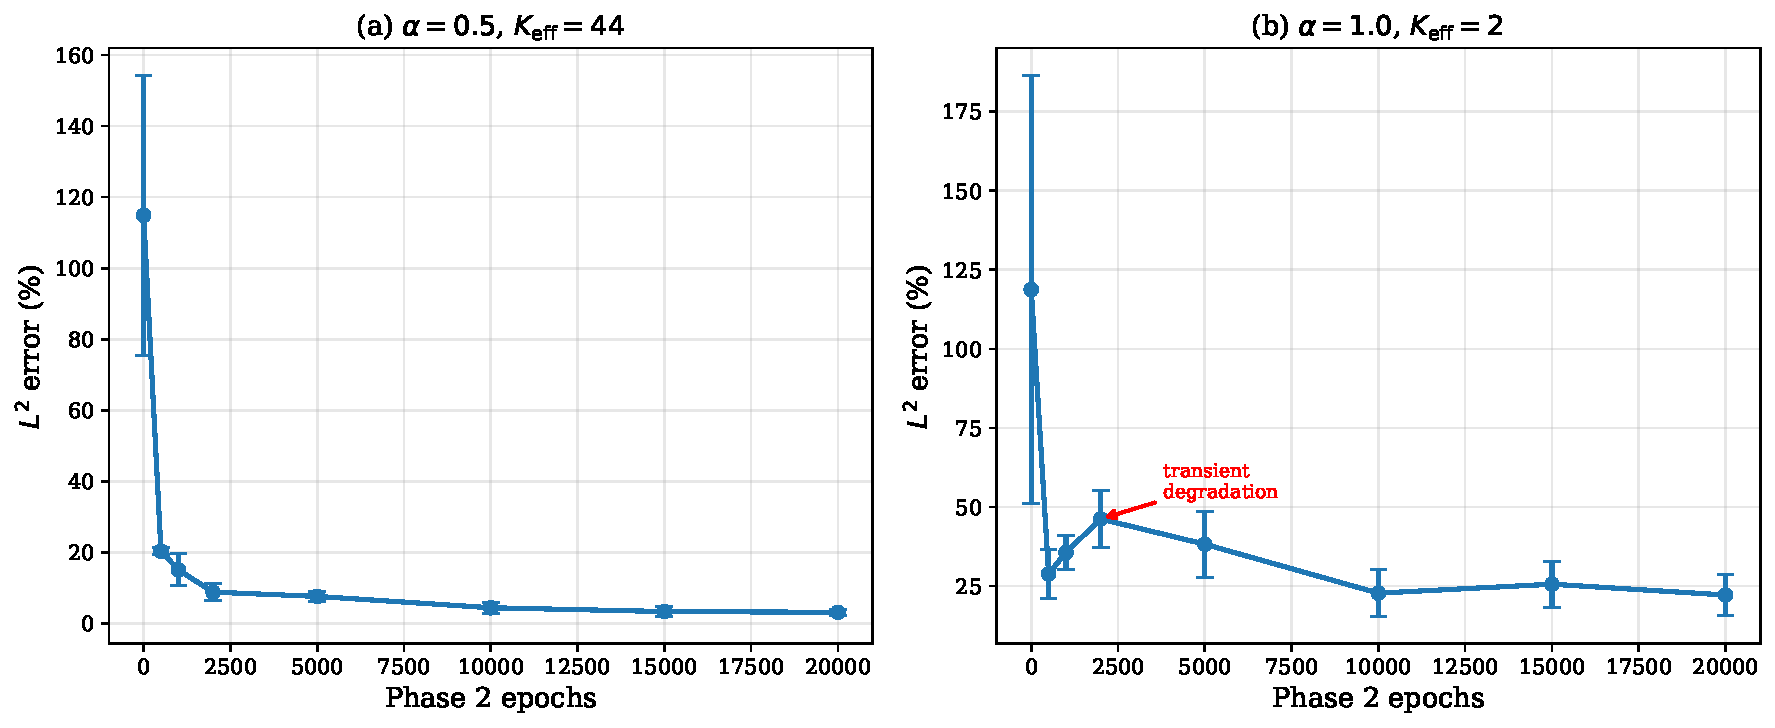
\includegraphics[width=\textwidth]{../figures/phase2_stability.pdf}
\caption{Phase~2 stability curves ($N_{\mathrm{terms}} = 20$, $\Ncol = 100$, 5 seeds). (a) $\alpha = 0.5$: monotonically stable ($114.9\% \to 3.1\%$). (b) $\alpha = 1.0$: transient degradation ($28.9\% \to 46.2\% \to 22.2\%$).}
\label{fig:phase2_stability}
\end{figure}

\textbf{Parametric characterization.} The two regimes are captured by:
\begin{itemize}
\item \emph{Stable} ($K_{\mathrm{eff}} \gg 2$): $L_2(e) \approx A\,\exp(-e/\tau) + B$. At $\alpha = 0.5$: $A \approx 108$, $\tau \approx 260$ epochs, $B \approx 6.3\%$.
\item \emph{Unstable} ($K_{\mathrm{eff}} \approx 2$): $L_2(e) \approx A\,\exp(-e/\tau_1) + C\,\exp\!\bigl(-((e-e_0)/\sigma)^2\bigr) + B$. At $\alpha = 1.0$: $A \approx 92$, $\tau_1 \approx 100$, $C \approx 31.5$, $e_0 \approx 3{,}172$, $\sigma \approx 2{,}101$, $B \approx 23.4\%$.
\end{itemize}

\textbf{GL-aware adaptive scheduling.} Scaling learning rate $\eta \propto \sqrt{K_{\mathrm{eff}}/2}$ and epoch budget $E \propto 1/\sqrt{K_{\mathrm{eff}}/2}$ yields the results in Table~\ref{tab:adaptive_phase2}.

\begin{table}[t]
\centering
\caption{GL-aware adaptive Phase~2 schedule vs.\ fixed schedule ($\Ncol = 100$, $N_{\mathrm{terms}} = 15$, 3 seeds). The adaptive schedule saves $2$--$3\times$ compute at low $\alpha$ with minimal accuracy loss at $\alpha \geq 0.9$.}
\label{tab:adaptive_phase2}
\begin{tabular}{ccccccc}
\toprule
$\alpha$ & $K_{\mathrm{eff}}$ & Fixed L2 (\%) & Adaptive L2 (\%) & Speedup & L2 ratio \\
\midrule
$0.5$ & $44$ & $6.73 \pm 2.24$ & $10.12 \pm 0.96$ & $3.3\times$ & $0.66\times$ \\
$0.7$ & $13$ & $9.64 \pm 3.69$ & $11.84 \pm 0.71$ & $2.6\times$ & $0.81\times$ \\
$0.9$ & $6$  & $13.74 \pm 5.07$ & $14.54 \pm 5.13$ & $1.7\times$ & $0.95\times$ \\
$1.0$ & $2$  & $28.52 \pm 13.33$ & $28.52 \pm 13.33$ & $1.0\times$ & $1.00\times$ \\
\bottomrule
\end{tabular}
\end{table}

The adaptive schedule reduces wall time by $3.3\times$ at $\alpha = 0.5$ at the cost of higher error ($10.1\%$ vs.\ $6.7\%$), but produces lower variance ($\pm 0.96$ vs.\ $\pm 2.24$). At $\alpha = 0.9$, accuracy loss is negligible ($0.95\times$).


\bibliographystyle{elsarticle-num}
\bibliography{references}

\end{document}
